\subsection{Temperatur}\label{subsec:Temperatur}
Um einen Einblick in das Temperaturverhalten des Motors zu erlangen, wurde in diesem Versuch die Erwärmung in Abhängigkeit der Drehzahl bei konstantem Moment gemessen. Die Messung erfolgte bei einer Drehzahl von 1550 RPM und bei 2550 RPM, und einem jeweiligen Drehmoment von 32Nm. Die Starttemperatur des Motors lag jeweils bei ca. 60°C und wurde solange betrieben, bis er eine Betriebstemperatur von 100°C erreicht hatte. Der Versuch in der Abbildung \ref{fig:Temperatur} wurde ohne zusätzliche Ventilation des Motors durchgeführt. Alle Versuche wurden gemäss den Bedingungen in Tabelle \ref{tab:Temperatur} durchgeführt.



\begin{table}[H]
	\centering
	\begin{tabular}{C{4cm} C{4cm} C{3cm}} 
		\multicolumn{3}{c}{\textbf{Versuchsbedingungen}} \\
		{Messgrösse}& {Bedingung} & {Wert}\\ \hline\hline 
		Spannung (DC)   & konstant &   96 V     \\
		Strom (DC)   & vernachlässigt &   -     \\
		Leistung (AC)   & vernachlässigt &   -    \\
		Drehzahl   & konstant &   1500/2500 RPM    \\
		Drehmoment-Sollwert   & konstant &   32 Nm    \\
		Motor-Temperatur   & gemessen &   40-100 °C    \\
		Controller-Temperatur   & gemessen &   35-64 °C    \\
	\end{tabular}
	\caption{Versuchsbedingungen Temperatur}\label{tab:Temperatur}
\end{table}

\begin{figure}[H]
	\centering
	\includegraphics[width=0.8\linewidth]{Temperatur.jpg}
	\caption{Erwärmung}\label{fig:Temperatur}
\end{figure}


Da die Leistung sowohl vom Drehmoment als auch von der Drehzahl abhängig ist, wurde  der Motor beim Versuch mit 2550 RPM und einer erhöhten Leistung betrieben, wodurch auch ein grössere Strom fliesst. Aus diesem Grund ist die Erwärmung des Motors bei höheren Drehzahlen dementsprechend grösser. In der Abbildung \ref{fig:TemperaturMotor} und \ref{fig:TemperaturController} sind der Temperaturverlauf des Motors und des Controllers ersichtlich. Beim Motor wurde zuerst die Messung mit nur einem zusätzlichen Ventilator (Anordnung hinter Motor) gemessen und anschliessend mit drei zusätzlichen Ventilatoren (Anordnung hinter und neben Motor). Beim Controller wurden ebenfalls zwei Messungen mit unterschiedlicher Kühlung durchgeführt. Die eine Messung mit einem grossen thermischen Kühlkörper (hier diente der Messtisch als Kühlkörper), die andere ohne Kühlkörper mittels thermischer Isolation zum Messtisch. Bei diesen Versuche wurde auch die Zeit zum Abkühlen gemessen, während die Drehzahl konstant bei 2500 RPM blieb.


\begin{figure}[H]
	\centering
	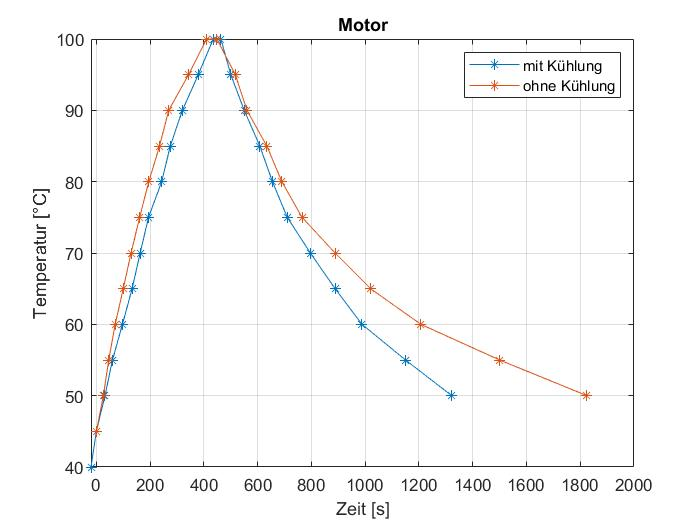
\includegraphics[width=0.8\linewidth]{TemperaturMotor.jpg}
	\caption{Temperaturverlauf Motor}\label{fig:TemperaturMotor}
\end{figure}

In der Temperaturkurve des Motors ist ersichtlich, dass die Zeit zum Abkühlen bedeutend grösser ist die der Erwärmung bei Nennmoment. Das der Motor im Abrollbetrieb mit einem hohen Wiederholungsintervall \ref{sec:Hardware} betrieben werden kann, muss der Motor zusätzlich gekühlt werden. Dasselbe verhalten ist auch beim Controller in nachfolgender Abbildung \ref{fig:TemperaturController} ersichtlich.

\begin{figure}[H]
	\centering
	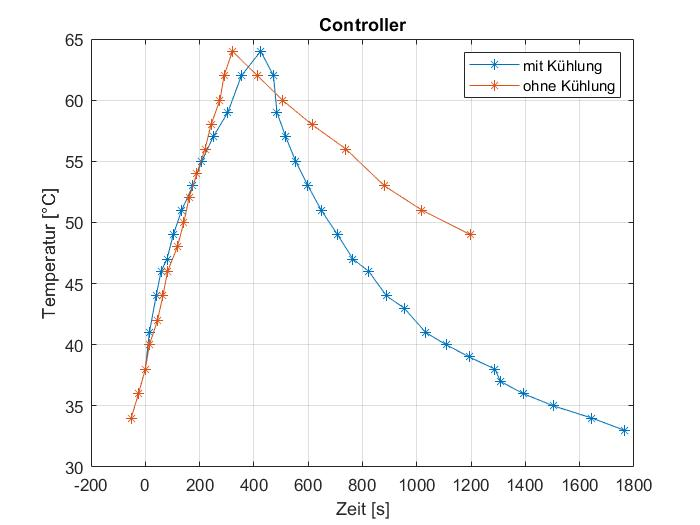
\includegraphics[width=0.8\linewidth]{TemperaturController.jpg}
	\caption{Temperaturverlauf Controller}\label{fig:TemperaturController}
\end{figure}

Es ist deutlich erkennbar, dass der Controller ohne Kühlung viel langsamer abkühlt. Der Hersteller weisst im Datenblatt jedoch keine max. Temperatur \cite{ControllerUserGuide} aus, weswegen wir eine Temperaturobergrenze von 65°C annehmen.